\batchmode
\documentclass[11pt]{book}
\makeatletter

\usepackage{epsfig}
\usepackage{html}
\usepackage{hypre}
\usepackage{makeidx}
\usepackage{graphicx}


\setlength{\oddsidemargin}{0in}
\setlength{\evensidemargin}{0in}
\setlength{\textwidth}{6.5in}
\setlength{\topmargin}{0in}
\setlength{\textheight}{8.0in}







\makeindex



\def\HYPREVersion{1.6.0}

\def\HYPREVersionDate{2001/07/27}

\def\pilut{{\sl PILUT}}

\makeatother
\newenvironment{tex2html_wrap}{}{}
\newwrite\lthtmlwrite
\def\lthtmltypeout#1{{\let\protect\string\immediate\write\lthtmlwrite{#1}}}%
\newbox\sizebox
\begin{document}
\pagestyle{empty}
\stepcounter{chapter}
\stepcounter{section}
\stepcounter{section}
\stepcounter{chapter}
\stepcounter{section}
\stepcounter{section}
{\newpage
\clearpage
\samepage \begin{figure}\centering
\includegraphics[width=5in]{concep_iface.eps}

\label{fig-conceptual-interface}
\end{figure}
}

\stepcounter{section}
\stepcounter{chapter}
{\newpage
\clearpage
\samepage \begin{figure}[t]
\centering
\includegraphics[width=4in]{fv_grid.eps}

\label{fig-fv-grid}
\end{figure}
}

{\newpage
\clearpage
\samepage \begin{equation}\label{eqn-laplacian}
\left \{
\begin{array}{ll}
\nabla^2 u = f , & \mbox{in the domain}, \\ 
u = 0,           & \mbox{on the boundary}.
\end{array}
\right .
\end{equation}
}

\stepcounter{section}
\stepcounter{section}
{\newpage
\clearpage
\samepage \begin{equation}\label{eqn-stencil-description}
\left [
\begin{array}{ccc}
        & ( 0, 1) &         \\ 
(-1, 0) & ( 0, 0) & ( 1, 0) \\ 
        & ( 0,-1) &        
\end{array}
\right ]
\equiv
\left [
\begin{array}{ccc}
    & S_4 &     \\ 
S_1 & S_0 & S_2 \\ 
    & S_3 &    
\end{array}
\right ] .
\end{equation}
}

{\newpage
\clearpage
\samepage \setbox\sizebox=\hbox{$S_0$}\lthtmltypeout{latex2htmlSize :tex2html_wrap_inline1373: \the\ht\sizebox::\the\dp\sizebox.}\box\sizebox
}

{\newpage
\clearpage
\samepage \setbox\sizebox=\hbox{$S_3$}\lthtmltypeout{latex2htmlSize :tex2html_wrap_inline1377: \the\ht\sizebox::\the\dp\sizebox.}\box\sizebox
}

\stepcounter{section}
{\newpage
\clearpage
\samepage \begin{equation}\label{eqn-stencil-laplacian}
\left [
\begin{array}{ccc}
    & -1 &    \\ 
 -1 &  4 & -1 \\ 
    & -1 &    
\end{array}
\right ] .
\end{equation}
}

\stepcounter{section}
\stepcounter{section}
{\newpage
\clearpage
\samepage \begin{equation}\label{eqn-symmetric-stencil}
\left [
\begin{array}{ccc}
 & ( 0, 1) &         \\ 
 & ( 0, 0) & ( 1, 0) \\ 
 &         &        
\end{array}
\right ]
\equiv
\left [
\begin{array}{ccc}
 & S_2 &     \\ 
 & S_0 & S_1 \\ 
 &     &    
\end{array}
\right ] .
\end{equation}
}

\stepcounter{chapter}
{\newpage
\clearpage
\samepage \begin{figure}[t]
\centering
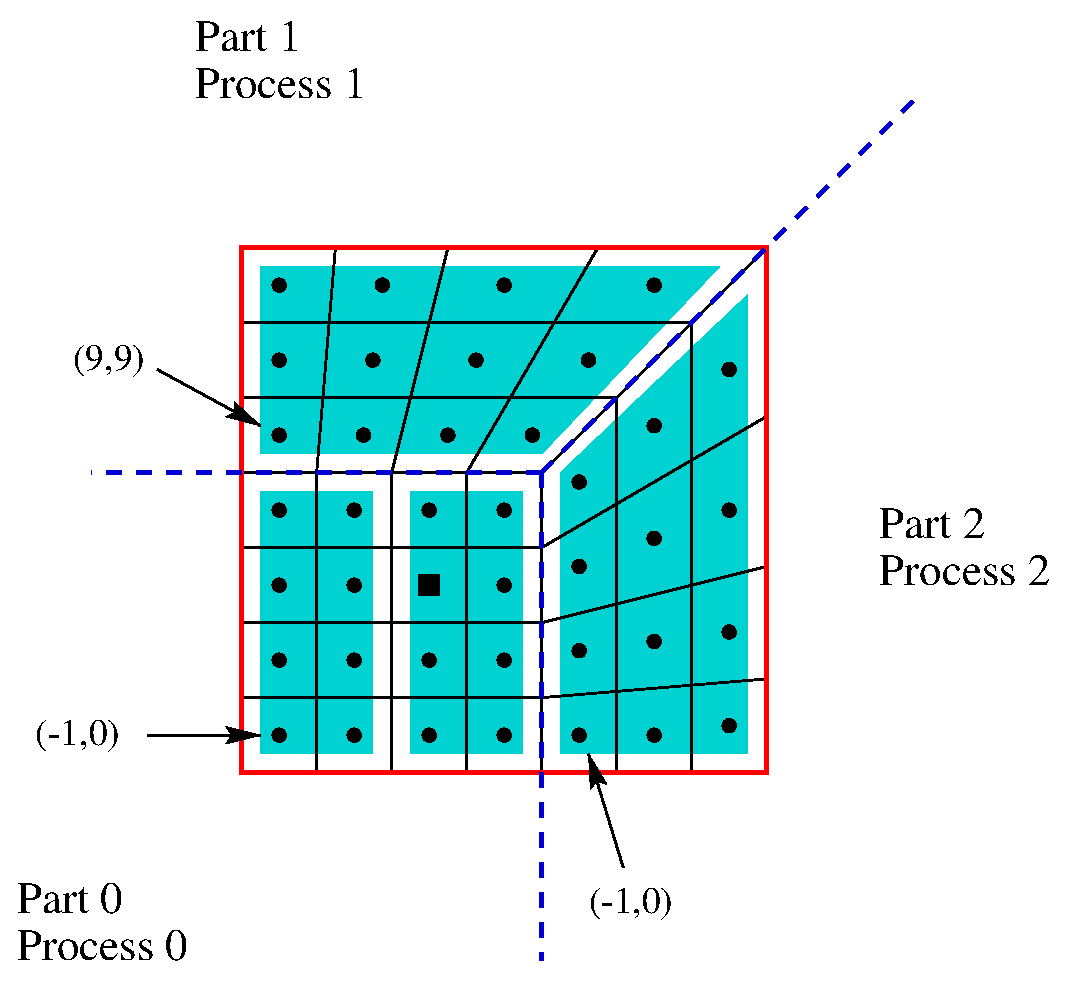
\includegraphics[width=4in]{block_structured.eps}

\label{fig-block-structured-grid}
\end{figure}
}

{\newpage
\clearpage
\samepage \begin{equation}\label{sstruct:eqn-laplacian}
\left \{
\begin{array}{ll}
\nabla^2 u = f , & \mbox{in the domain}, \\ 
u = 0,           & \mbox{on the boundary}.
\end{array}
\right .
\end{equation}
}

\stepcounter{section}
\stepcounter{section}
{\newpage
\clearpage
\samepage \begin{equation}\label{sstruct:eqn-stencil-description}
\left [
\begin{array}{ccc}
(-1, 1) & ( 0, 1) & ( 1, 1) \\ 
(-1, 0) & ( 0, 0) & ( 1, 0) \\ 
(-1,-1) & ( 0,-1) & ( 1,-1) 
\end{array}
\right ]
\equiv
\left [
\begin{array}{ccc}
S_7 & S_4 & S_8 \\ 
S_1 & S_0 & S_2 \\ 
S_5 & S_3 & S_6
\end{array}
\right ] .
\end{equation}
}

\stepcounter{section}
\stepcounter{section}
{\newpage
\clearpage
\samepage \begin{equation}\label{sstruct:eqn-stencil-laplacian}
\left [
\begin{array}{ccc}
 -1 & -1 & -1 \\ 
 -1 &  8 & -1 \\ 
 -1 & -1 & -1 
\end{array}
\right ] .
\end{equation}
}

\stepcounter{section}
\stepcounter{chapter}
\stepcounter{section}
\stepcounter{subsection}
\stepcounter{subsection}
{\newpage
\clearpage
\samepage \begin{table}[h]
\center
\begin{tabular}{|l|p{4.5in}|}
\hline
Parameter Name & Parameter Values \\ 
\hline\hline
solver &
\code{cg}, \code{gmres} (default), \code{bicgstab}, \code{tfqmr}, \code{boomeramg}, \code{superlu}, \code{superlux}
\\ 
preconditioner &
\code{diagonal} (default), \code{pilut}, \code{parasails}, \code{boomeramg}, \code{euclid}
\\ 
gmresDim &
an integer specifying the value of \code{m} in restarted GMRES(m).
The default value is 50.
\\ 
maxIterations &
an integer specifying the maximum number of iterations permitted for
CG or GMRES.  The default value is 1000.
\\ 
tolerance &
a floating point number specifying the termination criterion for CG or
GMRES.  The default value is 1.0E-10.
\\ 
pilutFillin &
an integer specifying the maximum number of nonzeros kept in the
formation of incomplete L and U.  If this is not called, a value will
be selected based on the sparsity of the matrix.
\\ 
pilutDropTol &
a floating point number specifying the threshold to drop small entries
in L and U.  The default value is 0.0.
\\ 
euclidNlevels &
a non-negative integer specifying the desired sparsity of the incomplete
factors. The default value is 0.
\\ 
euclidThreshold &
a floating point number specifying the threshold used to sparsify the 
incomplete factors. The default value is 0.0.
\\ 
superluOrdering &
\code{natural} (default) or \code{mmd} (minimum degree ordering).  This
ordering is used to minimize the number of nonzeros generated in the
LU decomposition.  The default is natural ordering.
\\ 
superluScale &
\code{y} (yes; perform row and column scalings before decomposition) or
\code{n} (no; default).
\\ 
amgCoarsenType &
\code{falgout}, \code{ruge}, or \code{default} (CLJP) coarsening for BoomerAMG.
\\ 
amgNumSweeps &
an integer specifying the number of pre- and post-smoothing at each
level of BoomerAMG.  The default is one pre- and one post-smoothings.
\\ 
amgRelaxType &
\code{jacobi} (Damped Jacobi), \code{gs-slow} (sequential Gauss-Seidel),
\code{gs-fast} (Gauss-Seidel on interior nodes), \code{hybrid}, or
\code{direct}. The default is \code{hybrid}.
\\ 
amgRelaxWeight &
a floating point number between 0 and 1 specifying the damping factor
for BoomerAMG's damped Jacobi smoother.  The default value is 0.5.
\\ 
amgStrongThreshold &
a floating point number between 0 and 1 specifying the threshold used
to determine strong coupling in BoomerAMG's coasening.  The default
value is 0.25.
\\ 
parasailsThreshold &
a floating point number between 0 and 1 specifying the threshold used
to prune small entries in setting up the sparse approximate inverse.
The default value is 0.0.
\\ 
parasailsNlevels &
an integer larger than 0 specifying the desired sparsity of the
approximate inverse.  The default value is 1.
\\ 
parasailsFilter &
a floating point number between 0 and 1 defining the threshold used to
prune small entries in A. The default is 0.0.
\\ 
parasailsLoadbal &
a floating point number between 0 and 1 specifying how load balancing has 
to be done. The default is 0.0.
\\ 
parasailsSymmetric &
set ParaSails to take A as symmetric.
\\ 
parasailsUnSymmetric &
set ParaSails to take A as nonsymmetric (default).
\\ 
parasailsReuse &
set ParaSails to reuse the sparsity pattern of A.
\\ 
\hline
\end{tabular}

\label{table-fei-param}
\end{table}
}

\stepcounter{chapter}
\stepcounter{section}
{\newpage
\clearpage
\samepage \begin{equation}\left[
\begin{array}{c}
~~~~~~~~~~ A_0 ~~~~~~~~~~ \\ 
A_1 \\ 
\vdots \\ 
A_{P-1}
\end{array}
\right]
\end{equation}
}

{\newpage
\clearpage
\samepage \setbox\sizebox=\hbox{$A_p$}\lthtmltypeout{latex2htmlSize :tex2html_wrap_inline1401: \the\ht\sizebox::\the\dp\sizebox.}\box\sizebox
}

\stepcounter{section}
\stepcounter{chapter}
{\newpage
\clearpage
\samepage \begin{table}[h]
\center
\begin{tabular}{|l||c|c|c|c|}
\hline
                               & \multicolumn{4}{|c|}{System Interfaces} \\ 
\multicolumn{1}{|c||}{Solvers} & Struct & SStruct & FEI & IJ \\ 
\hline\hline
Jacobi     & X &   &   &   \\ 
SMG        & X &   &   &   \\ 
PFMG       & X &   &   &   \\ 
BoomerAMG  &   & X & X & X \\ 
ParaSails  &   & X & X & X \\ 
Euclid     &   & X & X & X \\ 
PILUT      &   & X & X & X \\ 
PCG        & X & X & X & X \\ 
GMRES      & X & X & X & X \\ 
\hline
\end{tabular}

\label{table-solver-availability}
\end{table}
}

\stepcounter{section}
{\newpage
\clearpage
\samepage \begin{equation}\nabla \cdot ( D \nabla u ) + \sigma u = f
\end{equation}
}

\stepcounter{section}
\stepcounter{section}
\stepcounter{subsection}
\stepcounter{subsection}
{\newpage
\clearpage
\samepage \setbox\sizebox=\hbox{$\| b ~ - ~ Ax^{(n)} \|_2 / \| b \|_2 \leq $}\lthtmltypeout{latex2htmlSize :tex2html_wrap_inline1407: \the\ht\sizebox::\the\dp\sizebox.}\box\sizebox
}

{\newpage
\clearpage
\samepage \setbox\sizebox=\hbox{$10 ^{-7}$}\lthtmltypeout{latex2htmlSize :tex2html_wrap_inline1409: \the\ht\sizebox::\the\dp\sizebox.}\box\sizebox
}

{\newpage
\clearpage
\samepage \setbox\sizebox=\hbox{$-a_{i,j} \geq \theta 
\max_{j \neq i} \-a_{ij}$}\lthtmltypeout{latex2htmlSize :tex2html_wrap_inline1415: \the\ht\sizebox::\the\dp\sizebox.}\box\sizebox
}

{\newpage
\clearpage
\samepage \setbox\sizebox=\hbox{$\theta$}\lthtmltypeout{latex2htmlSize :tex2html_wrap_inline1417: \the\ht\sizebox::\the\dp\sizebox.}\box\sizebox
}

{\newpage
\clearpage
\samepage \begin{tabular}{l l}
  0 & CLJP-coarsening \\ 
  1& 	Ruge-Stueben coarsening without boundary treatment \\ 
  3& 	Ruge-Stueben coarsening with a 3rd 'second' pass on the boundaries \\ 
 6 & 	Falgout coarsening (default) \\ 
\end{tabular}
}

{\newpage
\clearpage
\samepage \begin{tabular}{l l}
 0 & weighted Jacobi \\ 
 1 & sequential Gauss-Seidel (very slow!) \\ 
 3 & Gauss-Seidel / Jacobi hybrid method (default) \\ 
 6 & symmetric Gauss-Seidel / Jacobi hybrid method \\ 
 9 & Gaussian elimination (only for the coarsest level (k=3), not recommended\\  
 & if the system on the coarsest level is large)\\ 
\end{tabular}
}

{\newpage
\clearpage
\samepage \begin{tabular}{l l}
 0 & no output (default) \\ 
 1 & matrix statistics (includes information on interpolation operators and \\ 
 & matrices generated on each level) \\ 
 2 & cycle statistics (includes residuals generated during solve phase) \\ 
 3 & matrix and cycle statistics \\ 
\end{tabular}
}

\stepcounter{section}
\stepcounter{subsection}
{\newpage
\clearpage
\samepage \setbox\sizebox=\hbox{$0 \le {\it thresh} \le 1$}\lthtmltypeout{latex2htmlSize :tex2html_wrap_inline1421: \the\ht\sizebox::\the\dp\sizebox.}\box\sizebox
}

{\newpage
\clearpage
\samepage \setbox\sizebox=\hbox{$0 \le {\it nlevels}$}\lthtmltypeout{latex2htmlSize :tex2html_wrap_inline1423: \the\ht\sizebox::\the\dp\sizebox.}\box\sizebox
}

{\newpage
\clearpage
\samepage \setbox\sizebox=\hbox{${\it thresh} = 0.1$}\lthtmltypeout{latex2htmlSize :tex2html_wrap_inline1425: \the\ht\sizebox::\the\dp\sizebox.}\box\sizebox
}

{\newpage
\clearpage
\samepage \setbox\sizebox=\hbox{${\it nlevels} = 1$}\lthtmltypeout{latex2htmlSize :tex2html_wrap_inline1427: \the\ht\sizebox::\the\dp\sizebox.}\box\sizebox
}

{\newpage
\clearpage
\samepage \setbox\sizebox=\hbox{$\tilde{A}^m$}\lthtmltypeout{latex2htmlSize :tex2html_wrap_inline1431: \the\ht\sizebox::\the\dp\sizebox.}\box\sizebox
}

{\newpage
\clearpage
\samepage \setbox\sizebox=\hbox{$\tilde{A}$}\lthtmltypeout{latex2htmlSize :tex2html_wrap_inline1433: \the\ht\sizebox::\the\dp\sizebox.}\box\sizebox
}

\stepcounter{subsection}
{\newpage
\clearpage
\samepage \begin{tabular}{|c|l|} \hline
value & meaning \\  \hline
0 & nonsymmetric and/or indefinite problem, and nonsymmetric preconditioner \\ 
1 & SPD problem, and SPD (factored) preconditioner \\ 
2 & nonsymmetric, definite problem, and SPD (factored) preconditioner \\  
\hline
\end{tabular}
}

{\newpage
\clearpage
\samepage \begin{tabular}{|c|c|c|c|c|l|} \hline
parameter    & type    & range                & sug. values  & default & meaning \\  \hline
{\tt nlevel} & integer & ${\tt nlevel} \ge 0$ & 0, 1, 2      & 1   & $m={\tt nlevel}+1$\\ 
\hline
{\tt thresh} & real    & ${\tt thresh} \ge 0$ & 0, 0.1, 0.01 & 0.1 & {\em thresh} $=$ {\tt thresh}\\ 
             &         & ${\tt thresh}  <  0$ & -0.75, -0.90 &     & {\em thresh} selected automatically\\ 
\hline
{\tt filter} & real    & ${\tt filter} \ge 0$ & 0, 0.05, 0.001 & 0.05 & filter value $=$ {\tt filter}\\ 
             &         & ${\tt filter}  <  0$ & -0.90        &     & filter value selected automatically\\ 
\hline
\end{tabular}
}

{\newpage
\clearpage
\samepage \setbox\sizebox=\hbox{${\tt thresh} < 0$}\lthtmltypeout{latex2htmlSize :tex2html_wrap_inline1457: \the\ht\sizebox::\the\dp\sizebox.}\box\sizebox
}

{\newpage
\clearpage
\samepage \setbox\sizebox=\hbox{$-{\tt thresh}$}\lthtmltypeout{latex2htmlSize :tex2html_wrap_inline1459: \the\ht\sizebox::\the\dp\sizebox.}\box\sizebox
}

{\newpage
\clearpage
\samepage \setbox\sizebox=\hbox{${\tt thresh} = -0.9$}\lthtmltypeout{latex2htmlSize :tex2html_wrap_inline1461: \the\ht\sizebox::\the\dp\sizebox.}\box\sizebox
}

{\newpage
\clearpage
\samepage \setbox\sizebox=\hbox{${\tt filter} < 0$}\lthtmltypeout{latex2htmlSize :tex2html_wrap_inline1467: \the\ht\sizebox::\the\dp\sizebox.}\box\sizebox
}

{\newpage
\clearpage
\samepage \setbox\sizebox=\hbox{$-{\tt filter}$}\lthtmltypeout{latex2htmlSize :tex2html_wrap_inline1469: \the\ht\sizebox::\the\dp\sizebox.}\box\sizebox
}

{\newpage
\clearpage
\samepage \setbox\sizebox=\hbox{${\tt filter} = -0.9$}\lthtmltypeout{latex2htmlSize :tex2html_wrap_inline1471: \the\ht\sizebox::\the\dp\sizebox.}\box\sizebox
}

\stepcounter{subsection}
{\newpage
\clearpage
\samepage \setbox\sizebox=\hbox{$(A+A^T)/2$}\lthtmltypeout{latex2htmlSize :tex2html_wrap_inline1479: \the\ht\sizebox::\the\dp\sizebox.}\box\sizebox
}

\stepcounter{section}
\stepcounter{subsection}
\stepcounter{subsection}
\stepcounter{subsection}
{\newpage
\clearpage
\samepage \setbox\sizebox=\hbox{$\langle int \rangle$}\lthtmltypeout{latex2htmlSize :tex2html_wrap_inline1491: \the\ht\sizebox::\the\dp\sizebox.}\box\sizebox
}

{\newpage
\clearpage
\samepage \setbox\sizebox=\hbox{$\langle float \rangle$}\lthtmltypeout{latex2htmlSize :tex2html_wrap_inline1495: \the\ht\sizebox::\the\dp\sizebox.}\box\sizebox
}

\stepcounter{section}
\stepcounter{chapter}
\stepcounter{section}
\stepcounter{subsection}
\stepcounter{subsection}
\stepcounter{section}
{\newpage
\clearpage
\samepage \begin{table}\center
\begin{tabular}{|l|l|}
\hline
C parameter & Fortran argument \\ 
\hline\hline
\code{int i} & \code{integer i} \\ 
\code{double d} & \code{double precision d} \\ 
\code{int *array} & \code{integer array(*)} \\ 
\code{double *array} & \code{double precision array(*)} \\ 
\code{char *string} & \code{character string(*)} \\ 
\code{HYPRE_Type object} & \code{integer*8 object} \\ 
\code{HYPRE_Type *object} & \code{integer*8 object} \\ 
\hline
\end{tabular}

\label{table-fortran-interface-types}
\end{table}
}

\stepcounter{section}
\stepcounter{chapter}

\end{document}
